% Some classes load the `subfigure` package which clashes with
% our internal use of `subfig` for subfloats. We are most likely
% not going to need the canned subfigure functionality anyways,
% so we'll trick LaTeX into thinking it already loaded `subfigure`
\makeatletter
\newcommand{\dontusepackage}[2][]{%
  \@namedef{ver@#2.sty}{9999/12/31}%
  \@namedef{opt@#2.sty}{#1}}
\makeatother
\dontusepackage{subfigure}


%% ===== Begin LaTeX file ===========================
%%
\documentclass[]{article}

\usepackage{lmodern}
\usepackage{amssymb,amsmath}
\usepackage{ifxetex,ifluatex}
\usepackage[usenames,dvipsnames]{color}
\usepackage{fixltx2e} % provides \textsubscript
\ifnum 0\ifxetex 1\fi\ifluatex 1\fi=0 % if pdftex
  \usepackage[T1]{fontenc}
  \usepackage[utf8]{inputenc}
  \usepackage{eurosym}
\else % if luatex or xelatex
  \ifxetex
    \usepackage{mathspec}
    \usepackage{xltxtra,xunicode}
  \else
    \usepackage{fontspec}
  \fi
  \defaultfontfeatures{Mapping=tex-text,Scale=MatchLowercase}
  \newcommand{\euro}{€}
\fi
% use upquote if available, for straight quotes in verbatim environments
\IfFileExists{upquote.sty}{\usepackage{upquote}}{}
% use microtype if available
\IfFileExists{microtype.sty}{%
\usepackage{microtype}
\UseMicrotypeSet[protrusion]{basicmath} % disable protrusion for tt fonts
}{}
\usepackage{listings}
% Define slightly more reasonable Listings defaults
\lstset{
    basicstyle=\ttfamily\small,
    breaklines=true,
    prebreak=\raisebox{0ex}[0ex][0ex]{\ensuremath{\hookleftarrow}},
    frame=lines,
    showtabs=false,
    showspaces=false,
    showstringspaces=false,
    keywordstyle=\color[gray]{0.4}\bfseries,
    commentstyle=\color[gray]{0.65}\itshape,
    numbers=left,
    captionpos=b,
}
\usepackage{graphicx}
\makeatletter
\def\maxwidth{\ifdim\Gin@nat@width>\linewidth\linewidth\else\Gin@nat@width\fi}
\def\maxheight{\ifdim\Gin@nat@height>\textheight\textheight\else\Gin@nat@height\fi}
\makeatother
% Scale images if necessary, so that they will not overflow the page
% margins by default, and it is still possible to overwrite the defaults
% using explicit options in \includegraphics[width, height, ...]{}
\setkeys{Gin}{width=\maxwidth,height=\maxheight,keepaspectratio}
\usepackage{caption}
\usepackage{float}
% Override extremely conservative LaTeX float placement rules
% (might need to be removed for "manuscript" styles)
\renewcommand{\topfraction}{0.85}	% max fraction of floats at top
\renewcommand{\bottomfraction}{0.75}	% max fraction of floats at bottom
\setcounter{topnumber}{2}
\setcounter{bottomnumber}{2}
\setcounter{totalnumber}{4}
\setcounter{dbltopnumber}{2}    % for 2-column pages
\renewcommand{\dbltopfraction}{0.85}	% fit big float above 2-col. text
\renewcommand{\textfraction}{0.10}	% allow minimal text w. figs
\renewcommand{\floatpagefraction}{0.85}	% require fuller float pages
\renewcommand{\dblfloatpagefraction}{0.85}	% require fuller float pages
% Encourage floats to be placed in the vacinity of where it is defined
% (in some manuscript styles where figures are collected at the end, the 'h'
% option might need to be removed by a separate '\floatplacement' call in the
% 'header-includes' metadata field)
\floatplacement{figure}{htbp}
\floatplacement{scholmdAlgorithm}{htbp}
\floatplacement{table}{htbp}
\ifxetex
  \usepackage[setpagesize=false, % page size defined by xetex
              unicode=false, % unicode breaks when used with xetex
              xetex]{hyperref}
\else
  \usepackage[unicode=true]{hyperref}
\fi
\hypersetup{breaklinks=true,
            bookmarks=true,
            pdfauthor={},
            pdftitle={},
            colorlinks=true,
            citecolor=black,
            urlcolor=blue,
            linkcolor=black,
            pdfborder={0 0 0}}
\urlstyle{same}  % don't use monospace font for urls
\setlength{\parindent}{0pt}
\setlength{\parskip}{6pt plus 2pt minus 1pt}
\setlength{\emergencystretch}{3em}  % prevent overfull lines
\setcounter{secnumdepth}{0}


\date{}


\begin{document}

\section{}\label{section}

title: Moton ajoneuvotietokoneen päivitysmahdollisuudet uudempaan
author: Tomi Haapaniemi subject: Moton ajoneuvotietokoneen
päivitysmahdollisuudet uudempaan date: 2015-03-31 company: Metropolia
AMK keywords: moto, sunit, ajoneuvopc ---

\title{Moton ajoneuvotietokoneen päivitysmahdollisuudet uudempaan}\date{\today}\author{Tomi Haapaniemi}

\maketitle

\newpage

\section{Lyhenteet}\label{lyhenteet}

x86: Yleisnimitys Intelin 1987 julkaisemalle
CISC-prosessorikäskykannalle. Alkuperäiset 8086/80186/80286 olivat
16-bittisiä, mutta 80386:sta eteenpäin käskykantaa laajennettiin
32-bittiseksi.

PS/2: Sarjaväyläinen, alunperin IBM PS/2 koneessa ollut
liitäntäprotokolla, joka yleistyi PC-koneiden standardiliitännäksi
näppäimistölle ja hiirelle ennen USB-protokollaa. 5V, GND, data, clock.

RS232: Alunperin v. 1962 esitelty asynkroninen sarjaliitäntäprotokolla,
joka oli ennen USB-liitännän yleistymistä yleisin PC-koneiden
oheislaitteiden liitäntäväylä.

USB: Universal Serial BUS, vuonna 1996 esitelty sarjaväyläinen liitäntä
oheislaitteiden liitäntään.

IDE/PATA: Integrated Drive Electronics (Parallel AT Attachments),
kiintolevyjen ja optisten asemien liittämiseen tarkoitettu 16-bittinen
rinnakkainen liitäntäväylä vuodelta 1986.

CAN: Controller Area Network, vikasietoinen, differentiaalinen
kaksijohtoinen automaatioväylä, jossa liikenne lähetetään priorisoituina
sanomina vuodelta 1986.

\section{Johdanto}\label{johdanto}

Tietokoneiden käyttöikä on varsinkin vaativissa kohteissa rajallinen.
Kun järjestelmien ikä kasvaa niin varaosien saatavuus vähenee. Viimein
ollaan pisteessä, missä ainoa vaihtoehto on korvata vanha järjestelmä
uudella. Tämä saattaa vaatia mittavia päivitysprojekteja myös
järjestelmää tukeviin kokonaisuuksiin ja vaihdon kannattavuus suhteessa
hyötyyn on huono.

Järjestelmänä on vuonna xxx valmistetun metsätraktori, eli
tuttavallisemmin moto. Motolla on n. yy v käyttöikää jäljellä ja moton
ajoneuvotietokone, jolla hallitaan koneen moottoriasetuksia, että myös
puiden kadon hallintaa, alkaa olemaan elinikänsä loppupäässä.
Alkuperäinen tietokone lakkaa toimimasta kokonaan kuumennettuaan liikaa,
kiintolevy on hajonnyt useaan otteeseen ja akustot alkavat olemaan
uusimisen tarpeessa. Jos laitteiston vaihtaisi kokonaan uudempaan olisi
kyseessä sen verran kallis toimenpide(n. 20 000\euro{}), ettei sitä
kannata tehdä enää kyseiseen metsätraktoriin. Tämän takia tutkimmekin
vaihtoehtoisia ratkaisuita lisätä metsätraktorin käytössä olevalle
tietokonejärjestelmälle elinikää.

Insinöörityön aiheena on löytää motossa käytetylle 15v vanhan Sunit
Nero-ajoneuvotietokoneelle korvaava uudempi, mutta yhteensopiva
tietokone. Tavoitteena on uuden laitteen yhteensopivuus vanhan
kiinnitysjärjestelmän kanssa, liitinyhteensopivuus, sekä ohjelmallisen
tason yhteensopivuus. Aluksi tutustutaan käytössä olevaan laitteistoon
ja sen asettamiin vaatimuksiin. Seuraavaksi käydään läpi mahdollisia
toteuttamisvaihtoehtoja ja niiden ominaisuuksia. Asennetaan uusi
ohjelmisto testikannetavaan ja testataan järjestelmä
tuotantoympäristössä. Lopuksi tutkitaan mahdolliset

Haasteita työlle asettavat vanhat ohjelmistot, tärinää ja pölyä ja
vaihtelevia lämpötiloja sisältävä työympäristö. Metsätraktori on
huoltoja lukuunottamatta metsässä kesät talvet ja lämpötilat vaihtelevat
talvella -20 asteesta +20 asteeseen ja kesäisin lämmöt voivat nousta
ohjaamossa jopa +50-60 asteeseen.

\chapter{Taustaa}\label{taustaa}

\section{Hakkuukoneet}\label{hakkuukoneet}

Hakkuukoneet eli motot (monitoimikoneet) ovat metsätraktoreita, joiden
tehtävänä on hakkuun kaikki työvaiheet. Hakkuukoneet sisältävät
tietokoneistetu mittalaitteet joilla katkonta ja mittaus saadaan
hoidettua tarkasti.

\subsection{Hakkuukone Valmet xxx}\label{hakkuukone-valmet-xxx}

Lorem ipsum dolor sit amet, consectetur adipiscing elit. Nam sed gravida
ex. Sed leo nisl, viverra in efficitur eget, imperdiet vel nibh. Donec
gravida sapien facilisis nisl rhoncus, sit amet ullamcorper nulla
congue. Donec egestas nisi sed finibus tempus. Integer convallis
suscipit magna et sollicitudin. Fusce gravida nisl eros, sit amet congue
odio aliquam vel. Vivamus congue massa eget est efficitur, dapibus
lacinia velit porttitor. Nunc consectetur sit amet augue vel ultrices.
Nullam hendrerit nisi efficitur tincidunt molestie.

\subsection{Motomit-mittalaite}\label{motomit-mittalaite}

Kohteena olevaan Valmet xxx-hakkuukoneeseen on jälkiasennettu Motomit-IT
-mittalaite, joka on korvannut hakkuukoneen alkuperäiset mittalaitteet
ja ohjelmiston hakkuussa. Motomit IT tukee StanForD-standardin mukaista
apteerausohjeiden tiedonsiirtoa. Motomit IT hoitaa sisäisen
kommunikaation CAN-väylää pitkin. Kommunikaatiossa alkuperäisen
ajoneuvotietokoneen kanssa käytetään RS232-väylää ja MotomitPC
-ohjelmistoa. (P. L. Oy 2008)

\subsubsection{Kuva: Motomit kaavio}\label{Motomitux5fkaavio}

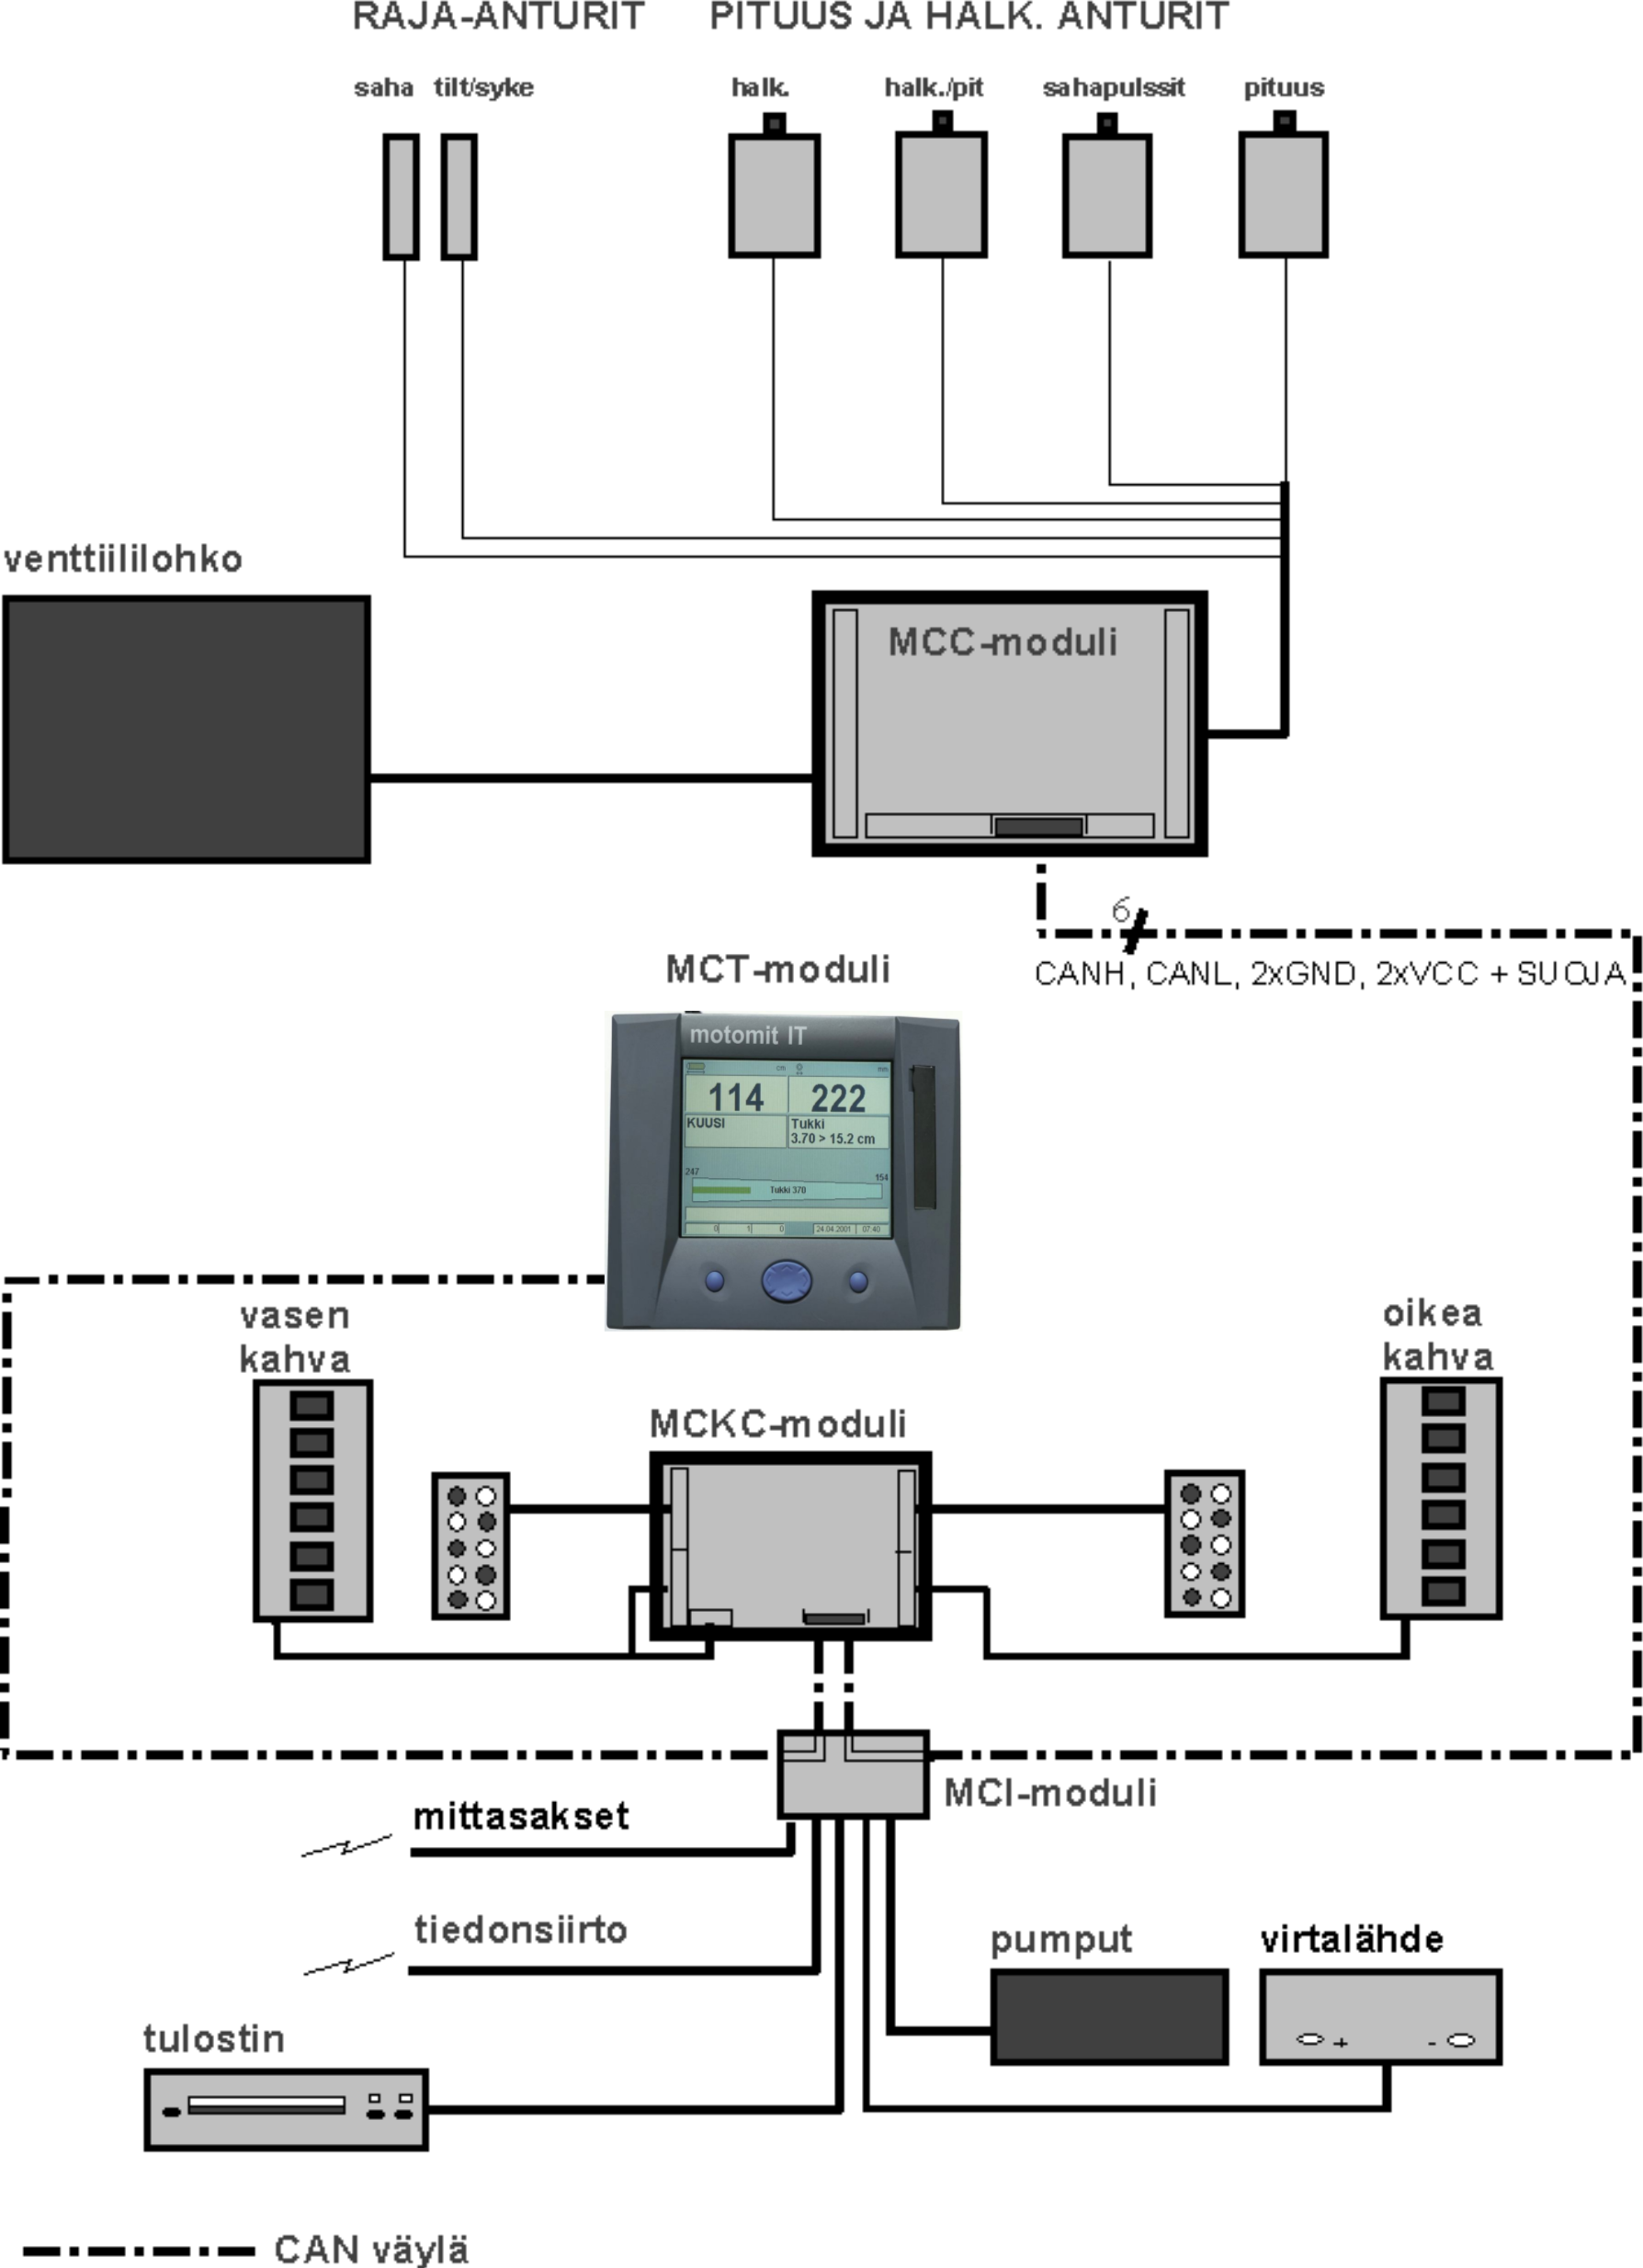
\includegraphics[width=1.000\textwidth]{../pictures/motomit_kaavio.png}
Caption: Motomit IT:n moduulikaavio

\section{Ajoneuvo-PC Sunit Nero / Valmet
Maxi}\label{ajoneuvo-pc-sunit-nero-valmet-maxi}

\begin{figure}
\centering
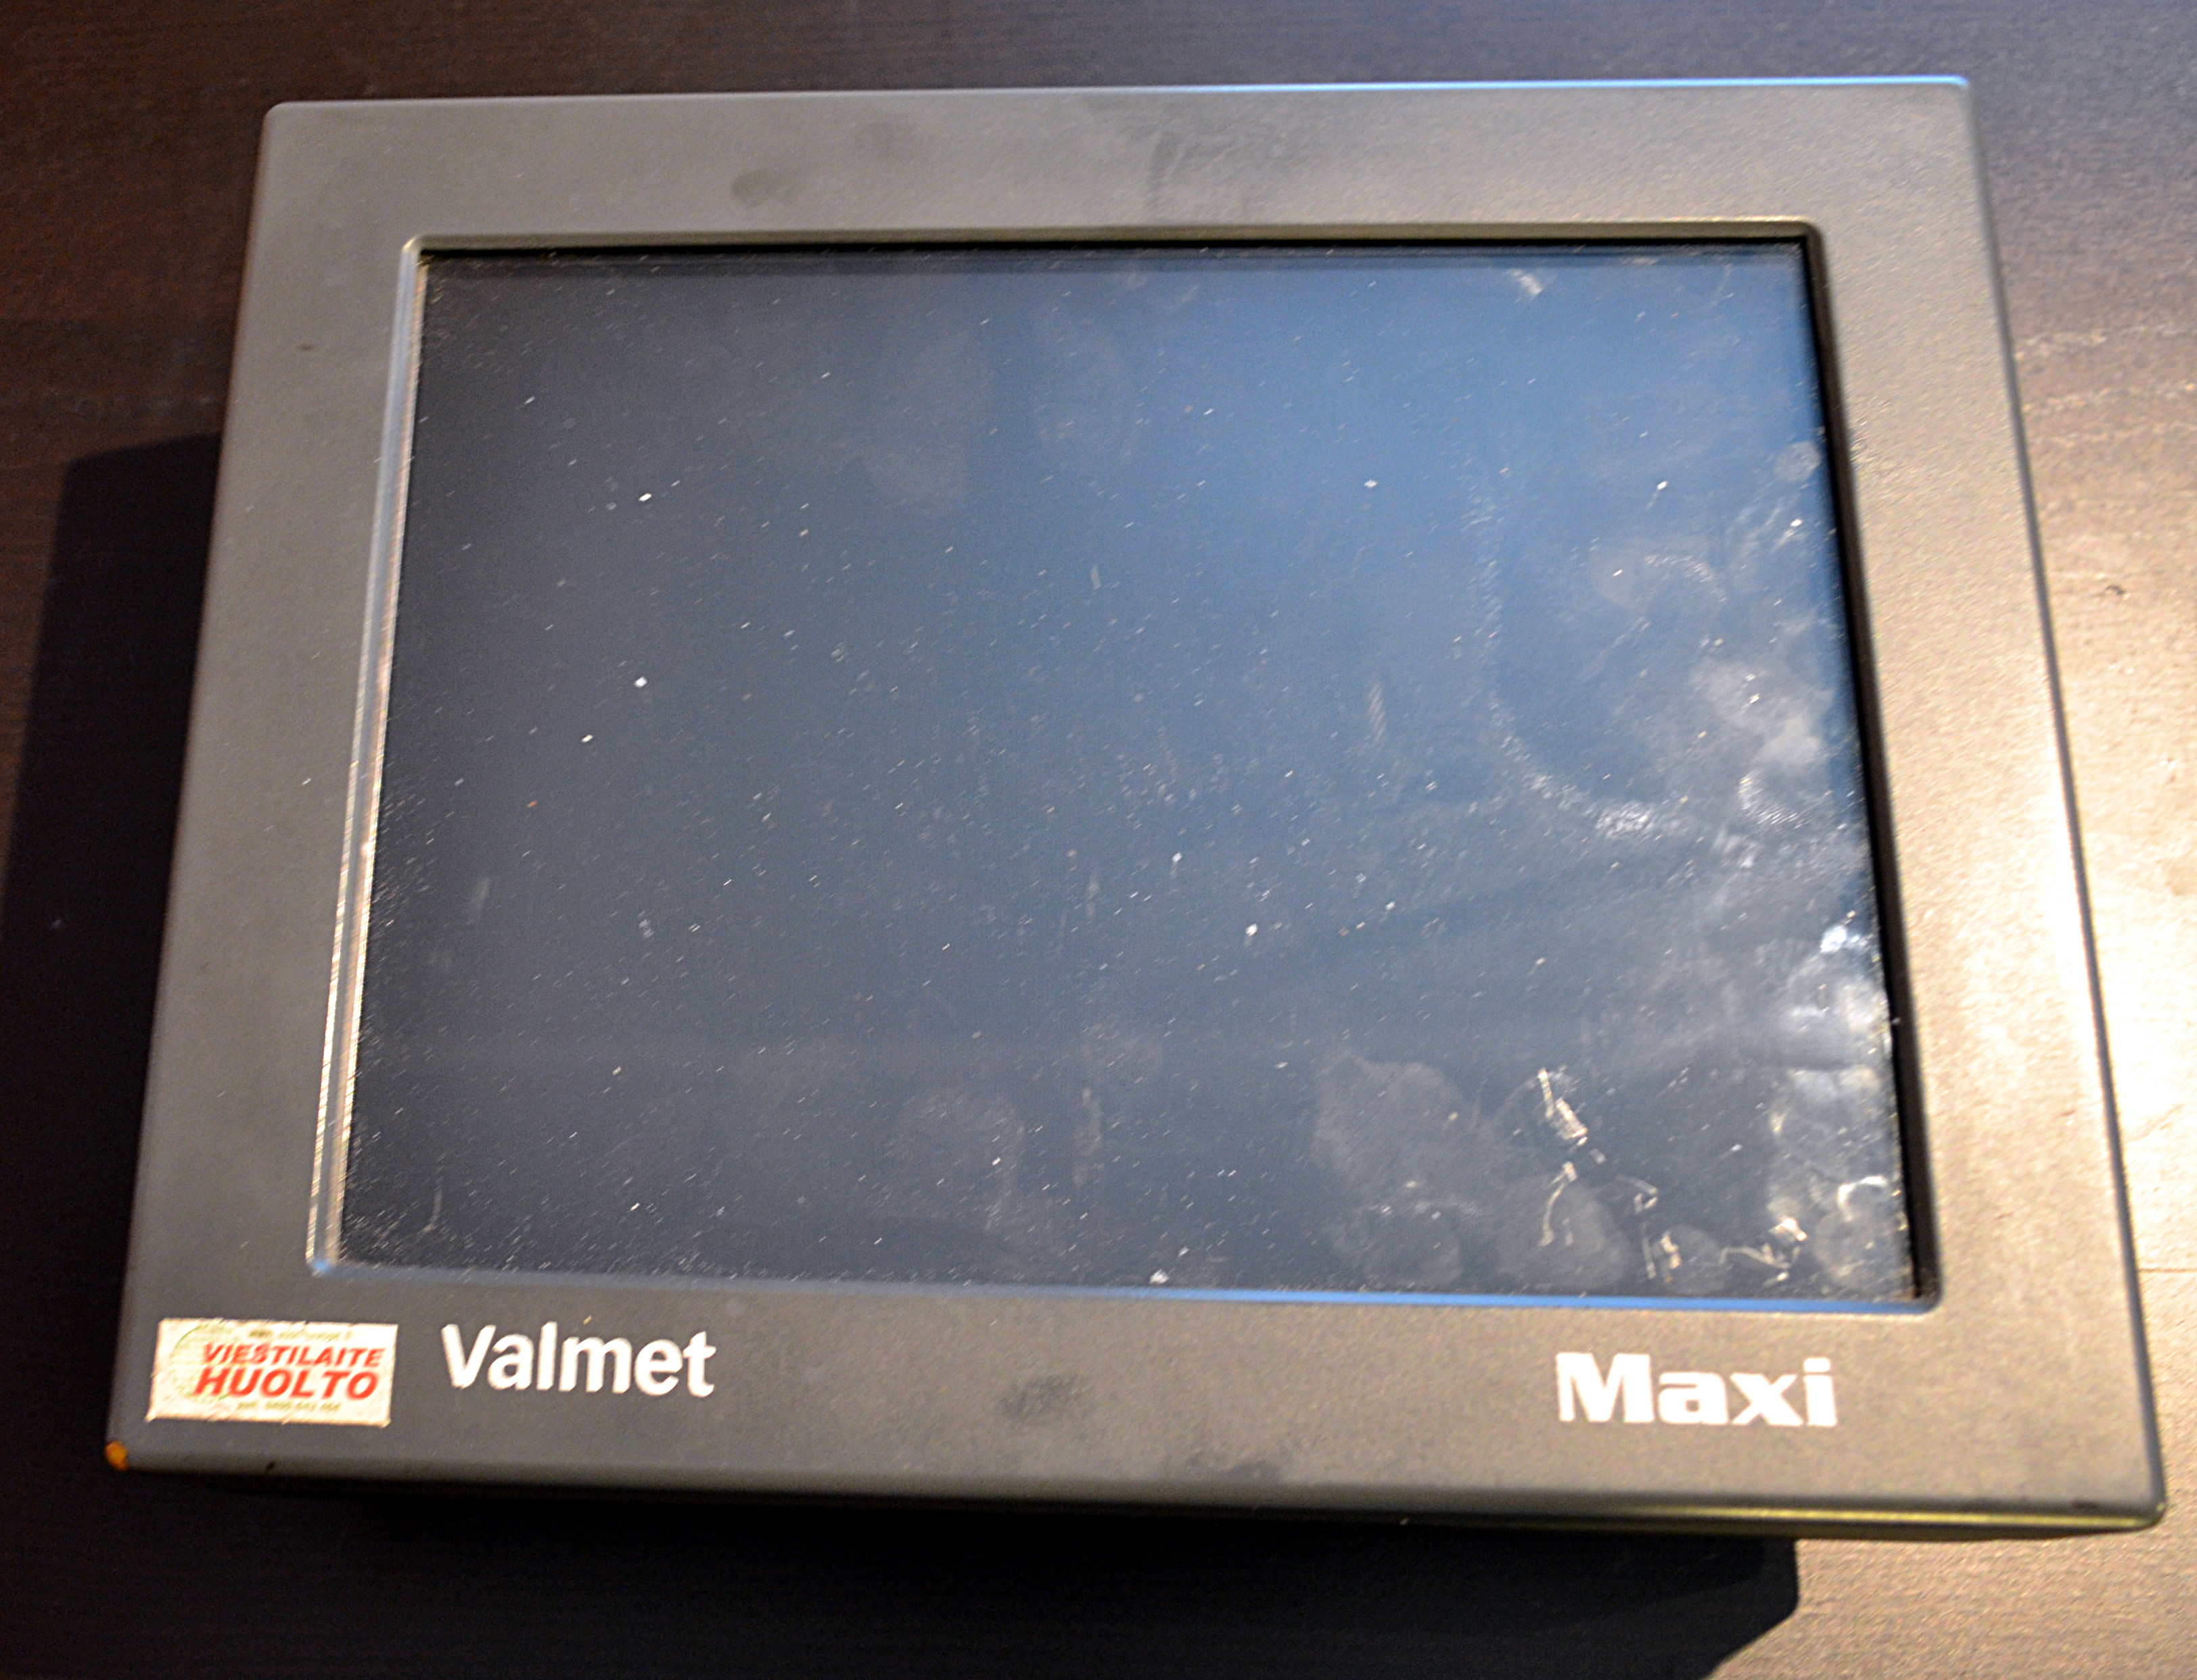
\includegraphics[width=1.000\hsize]{../pictures/valmet_maxi.jpg}
\caption{Hakkuukoneessa kiinni oleva ajoneuvo-PC Sunit Nero / Valmet
Maxi on valmistettu {[}joskus 1997-1999{]}. Sunit Nero on oikeastaan
kannettava, johon on modifioitu ulkopuoliset liittimet ja tukevampi
runko. Kotelointi koostuu XXX-muovisista ulkokuorista, sekä
metallilevystä (teräs? alumiini?), jonka molemmin puolin on komponentit
kiinnitetty. Toisella puolen on emolevy,prosessori,NIMH-akku (asetusten
säilytystä varten? ymmärtääkseni) ja liittimet, toisella puolen
kiintolevy, levykeasema,cd-asema ja näyttö. Näyttöpaneeli on 4:3 800x60
LCD.}\label{Nero}
\end{figure}

Ajoneuvotietokoneeessa on ollut koko käyttöiän (\textasciitilde{}15v)
erilaisia ongelmia. Alkuperäinen laite on vaihdettu syystä x vuonna y.
Nykyisestä laitteesta on kiintolevy hajonnut vuonna xxxx ja 2014,
jolloin pääsin ensimmäisen kerran tutustumaan laitteeseen paremmin.
Prosessori on vaihdettu v. zzzz.

\begin{figure}
\centering
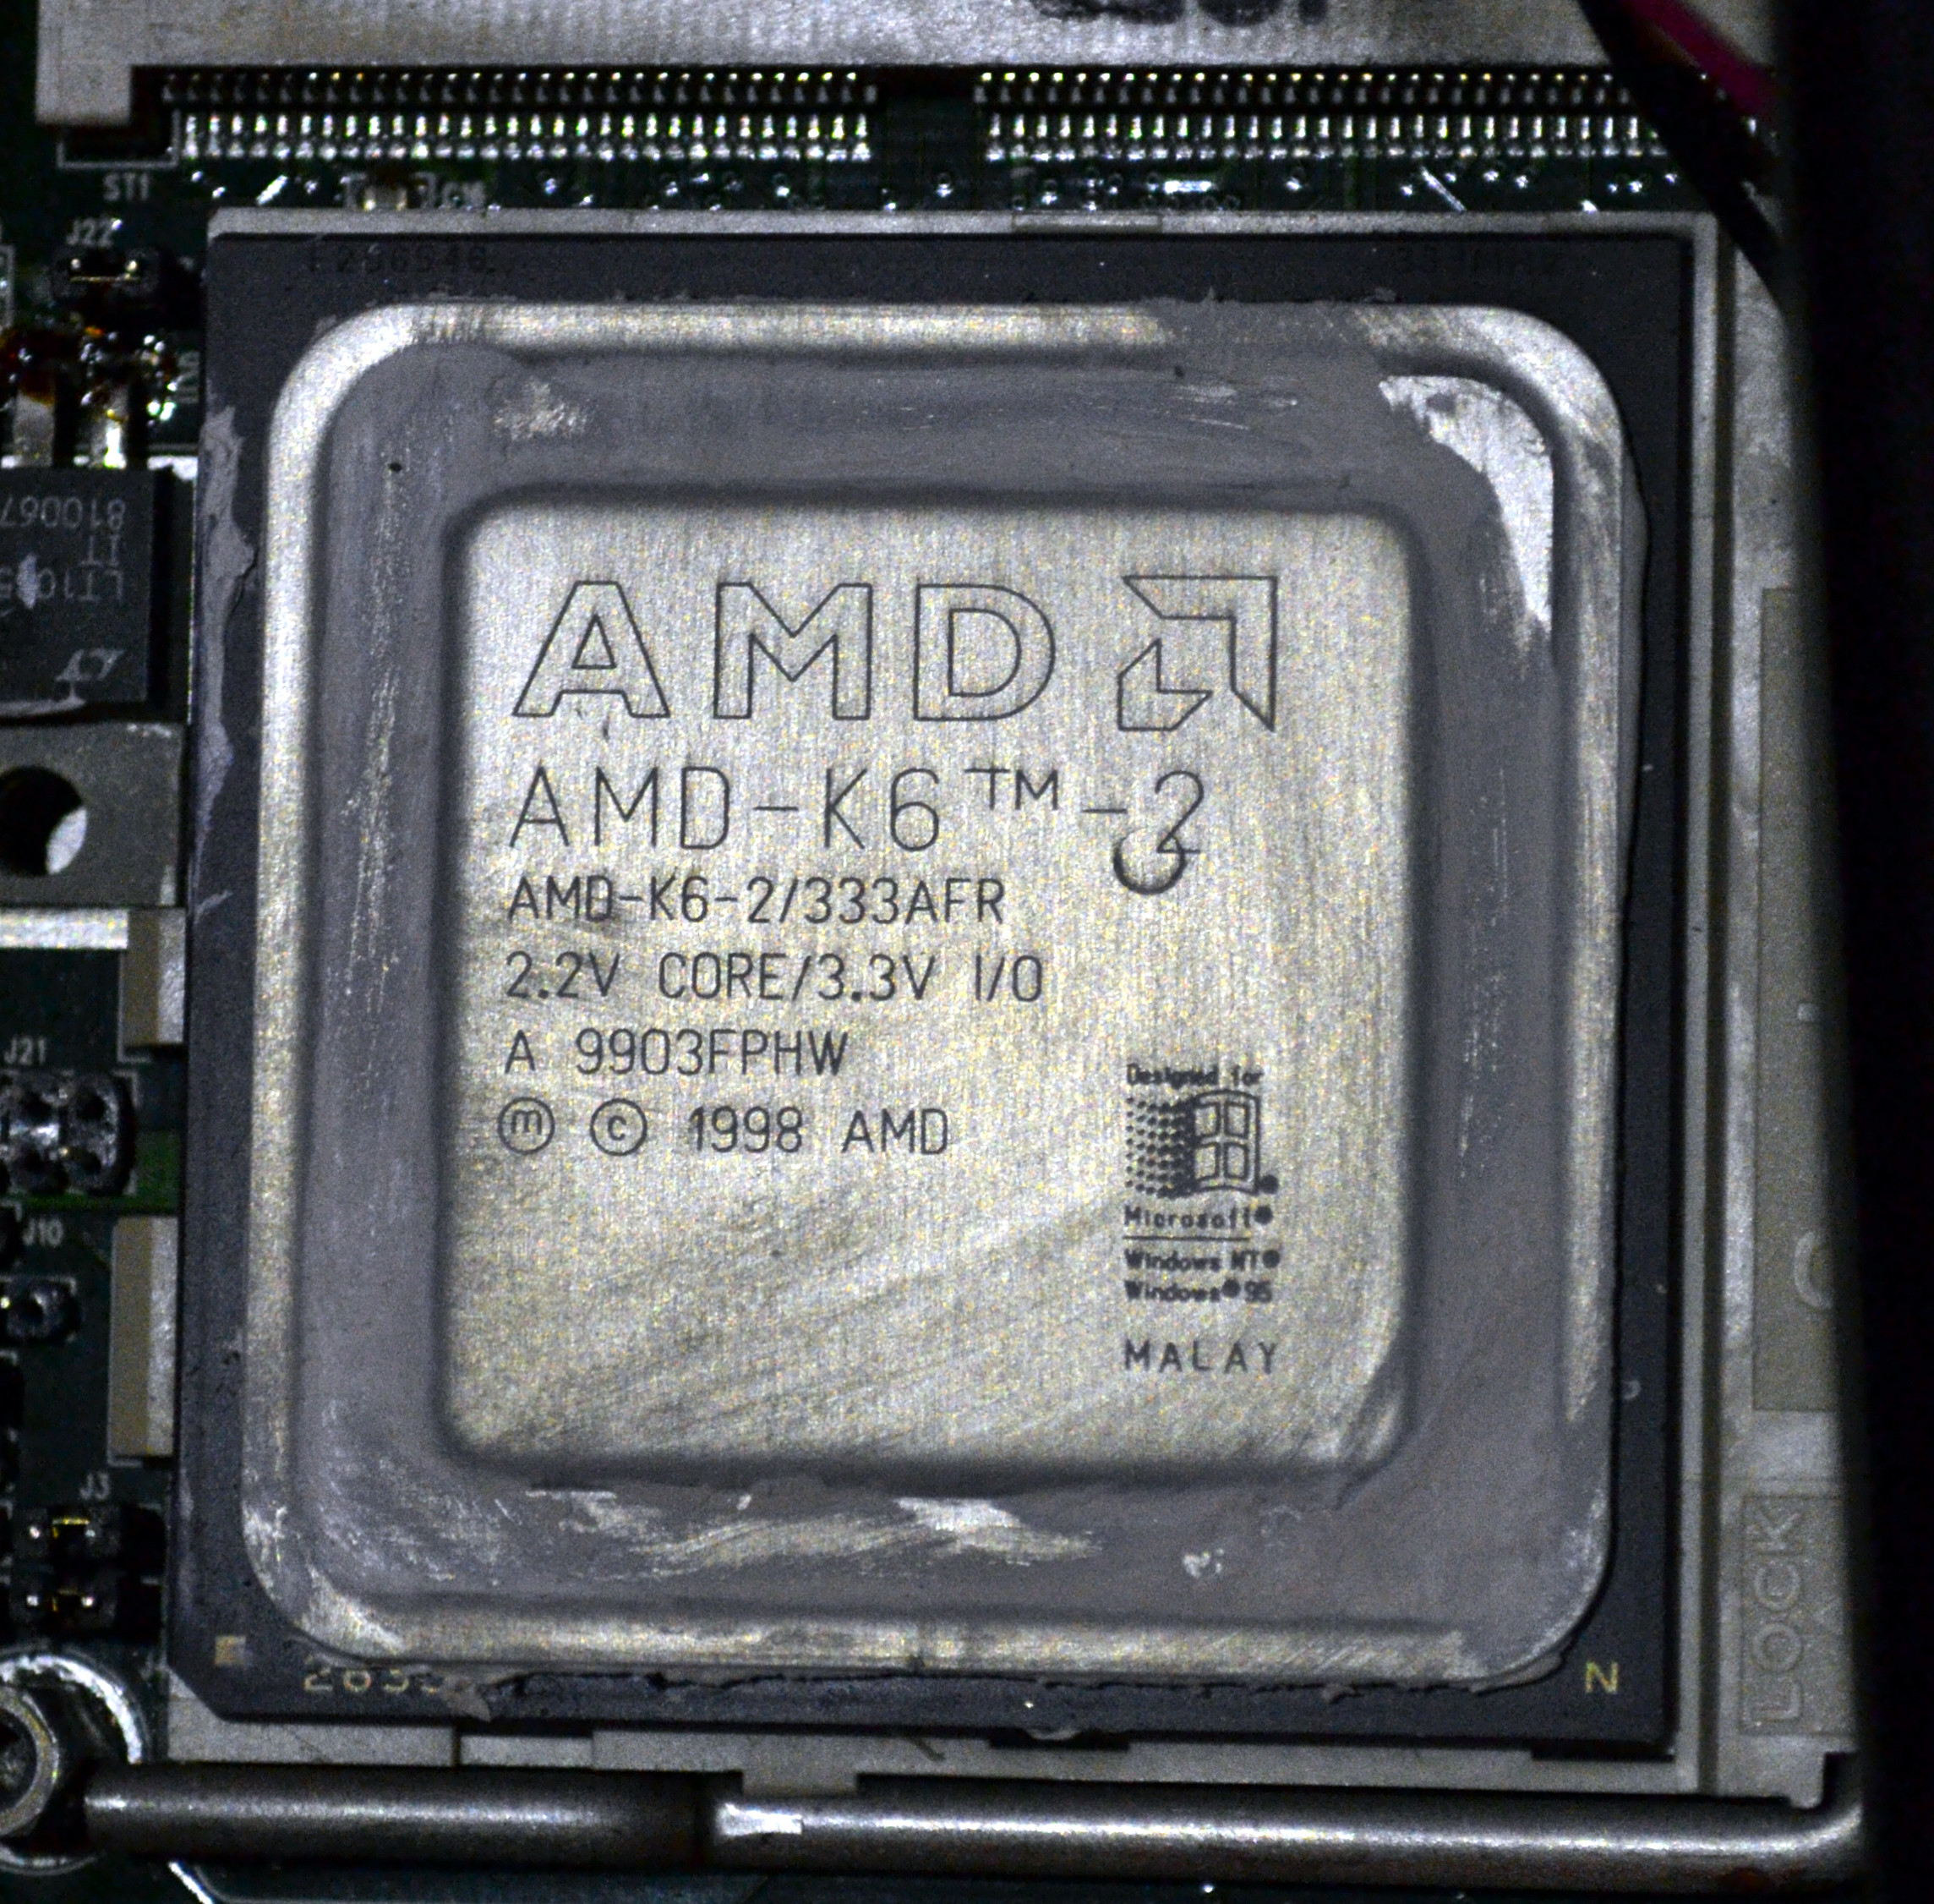
\includegraphics[width=0.500\hsize]{../pictures/processor.jpg}
\caption{AMD K6 66 MHz}\label{AMDK6}
\end{figure}

Koneen ongelmana on ollut viime aikoina ylikuumeneminen. Kuumennettuaan
siitä tulee epävakaa eikä se lähde päälle ennekuin jäähdyttyään, joka
kuumana kesäpäivänä traktorin hytissä vie aikaa

\section{Alkuperäinen
järjestelmä}\label{alkuperuxe4inen-juxe4rjestelmuxe4}

Lorem ipsum dolor sit amet, consectetur adipiscing elit. Proin tempus
vehicula aliquam. Morbi vulputate in lacus at convallis. Phasellus a
urna odio. Sed varius luctus imperdiet. Sed quis mollis nulla, non
posuere ipsum. Nunc elementum leo at ante molestie, sed fringilla nunc
luctus. Curabitur cursus mollis turpis eu ultrices. Nam id massa
sodales, congue ligula nec, scelerisque quam. Nunc ullamcorper massa
volutpat nibh rutrum, et convallis felis faucibus. Nunc vitae dolor sed
justo viverra malesuada. Duis luctus, lacus at bibendum varius, neque mi
feugiat quam, eget faucibus sapien tortor eget diam. Donec id libero
dapibus, interdum eros ac, euismod purus. Nam tincidunt at augue quis
mollis. Phasellus eget viverra neque. Integer felis purus, auctor
gravida varius vel, ultrices in risus. Proin nec aliquam nisl.

Ut eleifend tellus sit amet venenatis tincidunt. Quisque mattis interdum
augue, suscipit porta turpis cursus at. Sed suscipit ac urna eget
pretium. Suspendisse nisl justo, placerat vel urna et, luctus rutrum
arcu. Praesent maximus fringilla ante, ac vulputate urna dictum vel. Sed
non neque quis massa feugiat lacinia. Fusce eu mi posuere, volutpat
tortor ac, fermentum nulla. Sed id malesuada eros. Nulla eros est,
hendrerit in hendrerit sed, ultricies ac sem. Aliquam vel congue turpis.
Aenean viverra sagittis dolor vitae dapibus. Aenean ac tincidunt metus.
Curabitur in aliquet sem. Vestibulum ante ipsum primis in faucibus orci
luctus et ultrices posuere cubilia Curae;

\section{Standardeja}\label{standardeja}

\subsection{EU-direktiivi 2004/104/EY}\label{eu-direktiivi-2004104ey}

Direktiivi 2004/104/EY (Autoteollisuuden EMC-direktiivi) määrittää, että
1.7.2006 alkaen valmistettujen ajoneuvojen ja kiinteiästi asennetun
ajoneuvoelektroniikan aiheuttamat säteilypäästöt ja päästöjen sietokyky
mitataan kyseisen direktiivin mukaisesti. Direktiiviin on julkaistu
lisäys 2005/83/EY, joka tarkentaa direktiiviä. Uusi direktiivi korvaan
aiemman direktiivin 95/54/EY.

Uusi direktiivi vaatii tyyppihyväksynnän vain laitteilta, joilla on
vaikutusta ajoneuvon hallintaan, kuljettajan asennon muuttamiseen tai
kuljettajan näkyvyysalueeseen. Laitteiden, joiden ei tarvitse olla
tyyppihyväksyttyjä, pitää täyttää kuitenkin EMC-direktiivin 89/336/ETY
tai radio- ja telepäätelaitedirektiivin 1999/5/EY vaatimukset. (S. Oy
2006) {[}@1999/5/EY{]} {[}@89/336/ETY{]}

\subsection{EMC-direktiivi 89/336/ETY ja
2004/108/EY}\label{emc-direktiivi-89336ety-ja-2004108ey}

EMC-direktiivi 89/336/ETY määrittelee ainoastaan laitteistolta
vaadittavat ominaisuudet sähkömagneettisen yhteensopivuuden
takaamiseksi. Direktiivin tarkoitus on ohjeistaa valmistajia tekemään
elektromagneettisesti yhteensopivia laitteita. Direktiivi koskee kaikkia
sähkölaitteita ja -asennuksia, joita ei direktiivissä ole erikseen
rajattu sen ulkopuolelle {[}@89/336/ETY{]}. Direktiivi 2004/108/EY
kumosi vanhemman direktiivin 89/336/ETY 20.7.2004 alkaen. 2004/108/EY
mm. erotteli kiinteille asennuksille ja laitteille tehtävät asennukset,
sekä yksinkertaisti vaatimustenmukaisuuden arviointimenettelyä.
{[}@2004/108/EY{]}

\subsection{Radio- ja telepäätelaitedirektiivi
1999/5/EY}\label{radio--ja-telepuxe4uxe4telaitedirektiivi-19995ey}

Radio- ja telepäätelaitedirektiivi 1999/5/EY määrittää radio ja
telepäätelaitteiden yhteensopivuuden euroopan laajuisesti. Kaikkiin
direktiivin piiriin kuuluvien laitteiden tulee olla turvallisia
käyttäjälle ja muille henkilöille, sekä täyttää vaaditut
suojavaatimukset sähkömagneettisen yhteensopivuuden osalta. Lisäksi
direktiivi määrittää että laitteistojen tulee olla rakennettuja siten
että ne käyttävät tehokaasti radioviestintään varattua spektriä ja
resursseja. Tietyille laiteluokille on lisäksi määritelty vielä muita
vaadittuja lisäominaisuuksia, kuten yksityisyyden suojan takaamisen,
yhteensopivuuden muiden laitteistojen välillä, sisältävät petoksia
ehkäiseviä ominaisuuksia, tukevat hätäpalveluihin pääsyn takaavia
ominaisuuksia ja/tai sisältävät ominaisuuksia joilla laitteistojen
käyttö tehdään helpommaksi vammaisille {[}@1999/5/EY{]}. Direktiivi
1999/5/EY on kumottu 13.6.2016 alkaen direktiivillä 2014/53/EU
radiolaitteiden asettamista saataville markkinoilla koskevan
jäsenvaltioiden lainsäädännön yhdenmukaistamisesta. {[}@2014/53/EU{]}

\subsection{IP-suojaluokitus}\label{ip-suojaluokitus}

IP-suojaluokitus on standardissa IEC 60529 määritetty järjestelmä
sähkölaitteiden tiiveyden määrittämiseksi. IP-luokitus kertoo laitteiden
suojauksen pölyä ja vettä vastaan. (Maxim Integrated Products 2007)

\subsubsection{IP54}\label{ip54}

IP54-suojaluokitetut tuotteet ovat pölysuojattuja (ei täydellistä
tiiveyttä, mutta ei pölykertymiä), sekä roiskesuojattuja.

\subsubsection{IP67/66}\label{ip6766}

IP67/66 -suojaluokitetut tuotteet ovat täysin pölytiiviitä ja kestävät
suurella paineella tulevan vesiruiskun. IP67/66-tuotteet kestävät
tärinää ja iskuja 5M3-vaatimusten mukaisesti. (DIN EN 60721-3-5, MIL-STD
810F.)

\chapter{Tutustuminen alkuperäiseen
järjestelmään}\label{tutustuminen-alkuperuxe4iseen-juxe4rjestelmuxe4uxe4n}

\subsection{Huolto 05-06/2014}\label{huolto-05-062014}

Huoltaessani konetta 05-06/2014 vaihdoin kiintolevyn, sekä uudet
lämpötahnat prosessorille. Kiintolevyn vaihdon takia emolevy piti
irroittaa kiinnitysruuvien sijainnin takia ja samalla myös
prosessorijäähy. Vanhat jäähdytyslevyn lämpötahnat olivat kuivaneet ja
vaihdoin tilalle hopeatahnaa jota löytyi varastostani. Kiintolevyn
hankin käytettynä Huuto.netistä koska uusien toimitusajat olivat
viikkoja, hinnat \textasciitilde{}100\euro{} eikä kiintolevyn koolla
ollut väliä koska kyseessä on minimaallinen ohjelmien ja tilantarve.

Kone kiinnitettiin takaisin motoon 1.7.2014 ja säädettyä portit kuntoon
MotomitPC:stä ja Termanista, järjestelmä vaikutti toimivan ja poistuin
paikalta. \#\#\#\# Figure: Moto \{\#Moto1\}
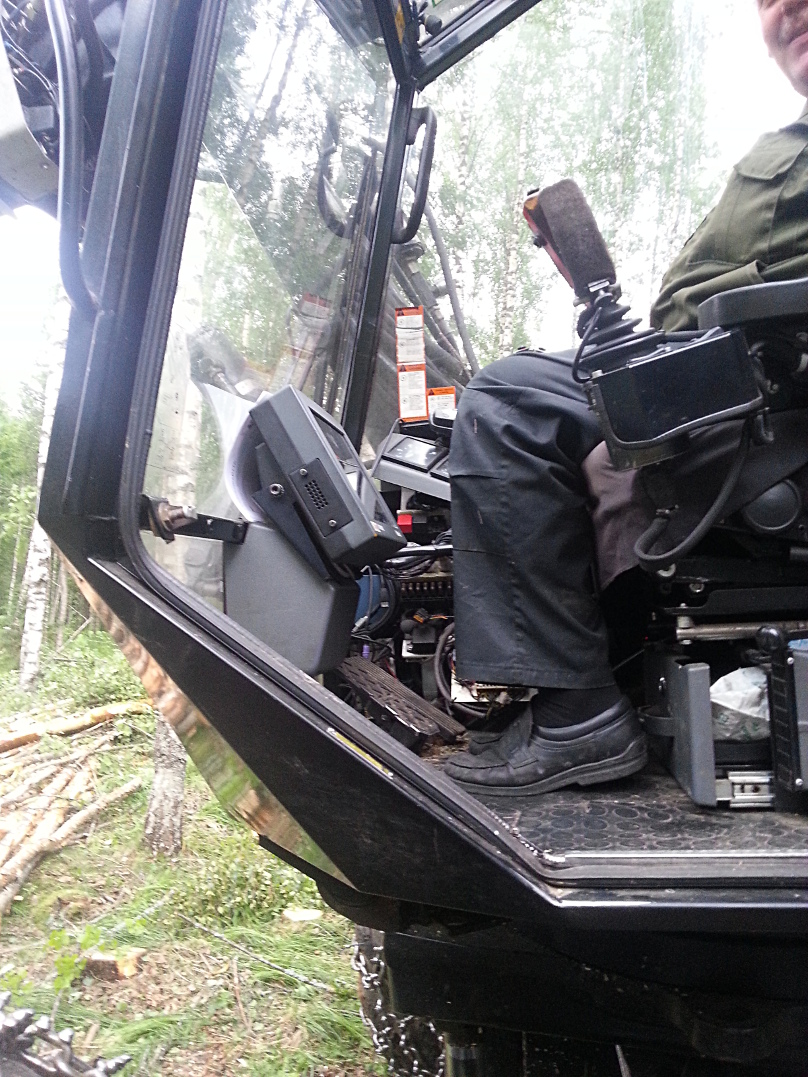
\includegraphics[width=0.250\textwidth]{../pictures/moto_1.jpg}
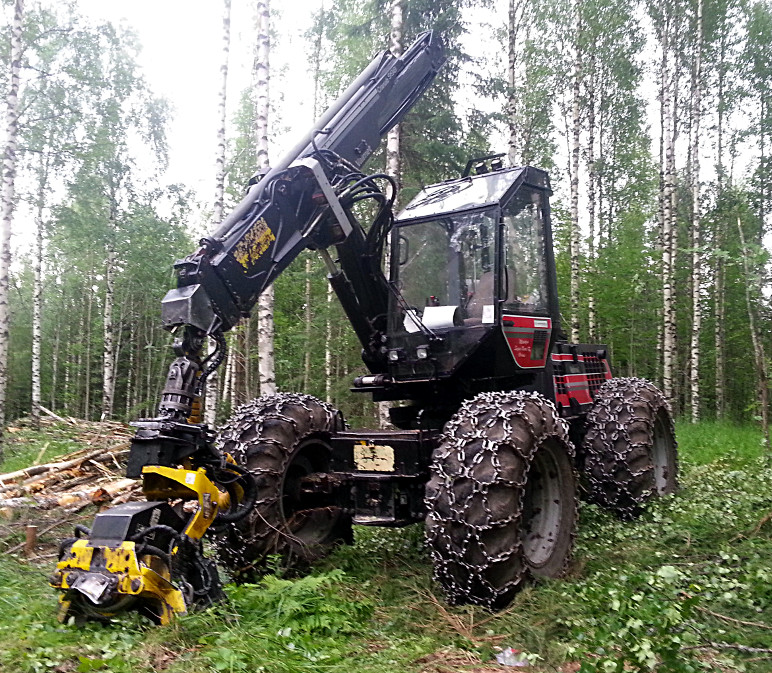
\includegraphics[width=0.250\textwidth]{../pictures/moto_2.jpg}

\subsection{Huolto xx/2014}\label{huolto-xx2014}

Vaihdettu, käytettynä ostettu kiintolevy oli hajonnut käytössä ja se
korvattiin SD-muistikorttipohjaisella ratkaisulla.

\subsection{Huolto 03/2015}\label{huolto-032015}

Koneen BIOS-asetuksia ylläpitävä akusto (NIMH 10,8V) hajosi ja
tietokoneen hukattua asetukset se ei enää suostunut käynnistymään
normaalisti. Akku vaihdettiin/uudelleenkennotettiin, ja
SD-muistikortilla oleva käyttöjärjestelmä+ohjelmisto varmuuskopioitiin.

Maecenas at faucibus libero, ut consequat felis. Curabitur blandit arcu
at velit mattis, at sagittis felis egestas. Integer massa lacus,
efficitur a blandit eget, imperdiet a velit. Curabitur viverra elit quis
mauris tincidunt ornare. Cum sociis natoque penatibus et magnis dis
parturient montes, nascetur ridiculus mus. Pellentesque pharetra, orci
eu commodo mattis, tellus nisi tristique lectus, id pellentesque nisi
risus eu nisi. Morbi aliquam neque a lectus tincidunt euismod a sagittis
dui. Pellentesque eu dapibus dui, eget porttitor risus. Aliquam
porttitor laoreet libero sed elementum. Phasellus blandit eget ipsum sit
amet consequat. Nulla ut nisl mollis nunc dapibus malesuada sit amet
suscipit erat. Curabitur lobortis eget mauris in condimentum. Donec
finibus, odio sit amet condimentum condimentum, mauris nulla egestas
nulla, vel aliquet felis odio nec orci. Sed dapibus feugiat nisi, sit
amet maximus velit iaculis ac.

\chapter{Suunnittelu}\label{suunnittelu}

\section{Toteuttamisvaihtoehdot}\label{toteuttamisvaihtoehdot}

\subsection{Natiivi ympäristö}\label{natiivi-ympuxe4ristuxf6}

Vaihtoehdossa tietokoneeseen asennettaan uusin käyttöjärjestelmä, mitä
käytössä oleva laitteisto ja ohjelmat tukevat. Vaihtoehto on
haasteellinen, koska ohjelmistot ovat vanhoja ja laitteisto uutta.
Uusien laitteiden tuki vanhoilla käyttöjärjestelmillä on puutteellinen
tai puuttuva.

\subsection{Ohjelmistojen rajapintojen
yhteensopivuuskerros}\label{ohjelmistojen-rajapintojen-yhteensopivuuskerros}

Vaihtoehdossa käytetään käyttöjärjestelmän ja ohjelman välissä sopivia
rajapintakerroksia, jolloin saadaan käyttöjärjestelmän kanssa
yhteensopimattomat ohjelmat toimimaan keskenään. Vaihtoehto vaatii
yhteensopivan laitteistoarkkitehtuurin alkuperäisen järjestelmän kanssa.
Nykyiset Windows-versiot (Windows XP+) sisältävät jo valmiiksi
yhteensopivuustilan, joka mahdollistaa vanhempien ohjelmien käyttämisen
uudemmissa käyttöjärjestelmissä. Linuxissa Wine-rajapintatoteutus
mahdollistaa kaikenikäisten Windows-sovellusten ajamisen Linuxissa.

\subsection{Virtualisointi}\label{virtualisointi}

Vaihtoehdossa alkuperäisiä ohjelmistoja+käyttöjärjestelmää ajetaan
virtuaalikoneessa toisen käyttöjärjestelmän päällä. Näin saavutetaan
varmin yhteensopivuus ohjelmistotasolla. Oheislaitteiden siirtämisessä
virtualisoidun koneen käyttöön on rajoituksia, jotka pitää huomioida
virtualisointiohjelmistoja valittaessa. Vaihtoehto kuluttaa muistia
enemmän ja on hieman hitaampi kuin natiivi toteutus, hyötysuhteen
ollessa \textasciitilde{}90\% natiivista (anandtech 2009).

\subsection{Järjestelmäemulointi}\label{juxe4rjestelmuxe4emulointi}

Vaihtoehdossa alkuperäisiä ohjelmistoja+käyttöjärjestelmä ajetaan
emulaattorissa toisen järjestelmän päällä. Emuloimalla saavutetaan
laitteistoarkkitehtuuririippumattomuus isäntäkoneen ja emuloitavan
järjestelmän välillä. Emuloinnin haittapuolena on hitaus. Nyrkkisääntönä
on 20\% hyötysuhde (Landley and Miller 2010), parhaat emulaattorit
pääsevät n. 40\% hyötysuhteeseen {[}@40pperf{]}

\subsection{Ohjelmistojen emulointi}\label{ohjelmistojen-emulointi}

Vaihtoehdossa emuloidaan vain ohjelmat koko pc:n sijasta. Tämä onnistuu
tietyillä ohjelmilla tiettyjen ohjelmistoarkkitehtuurien välillä
(Liguori 2010),(Landley and Miller 2010). Vaihtoehdolla voi ajaa
x86-ohjelmia ARM-prosessoreilla.

\subsection{Valinta}\label{valinta}

X86: Lorem ipsum dolor sit amet, consectetur adipiscing elit. Nunc
vestibulum magna dui, quis vestibulum libero molestie vel. Phasellus dui
risus, vehicula sit amet tincidunt nec, rutrum at erat. Aenean ex dolor,
luctus sit amet scelerisque vel, euismod vel urna. Morbi accumsan, odio
at tincidunt cursus, nibh quam consectetur turpis, at ultrices erat
lorem tristique libero. Fusce aliquet lectus sit amet sodales convallis.
Proin tempor libero eu accumsan bibendum. Proin ullamcorper tempor eros,
blandit pellentesque eros ornare vel. Nulla ac ultricies nisi. Phasellus
ligula lectus, ullamcorper in libero sit amet, pretium pretium dolor.
Nunc euismod mollis nibh, at rhoncus dolor volutpat blandit. Nam ipsum
felis, tempus ut justo ut, fringilla tincidunt augue. Vivamus non
finibus turpis, at consectetur justo.

Pellentesque ullamcorper odio at arcu venenatis consequat vel at sem.
Nulla sed scelerisque justo. Nunc consequat sem nunc, a maximus mi
ultrices non. Nunc posuere eu sapien a laoreet. Quisque sit amet mi
congue, tempus libero ut, viverra velit. Donec aliquam, metus non
rhoncus ullamcorper, magna quam pharetra lectus, in dapibus sapien
sapien quis purus. Maecenas convallis luctus semper. Nunc non ex nec est
faucibus faucibus ac eget dui. Phasellus ligula urna, lacinia in metus
nec, bibendum lobortis leo. Nunc dictum urna tortor, nec viverra dolor
suscipit et. Pellentesque vel hendrerit elit, eu pharetra quam. Cras
fringilla ullamcorper massa, quis porta justo. Praesent cursus, elit nec
finibus convallis, felis lorem luctus nulla, ut pulvinar tellus quam
feugiat turpis. Donec hendrerit massa eu ornare scelerisque. Cras non
elit vitae risus scelerisque mollis. Pellentesque vehicula sapien nec
felis eleifend blandit sit amet eu magna.

\chapter{Toteutus}\label{toteutus}

Projektissa päädyttiin käyttämään käyttöjärjestelmänä
Linux-distribuutiota Xubuntu 14.04. Alkuperäiset ohjelmistot Motomit PC
ja Terman sovitettiin käyttöön Wine-rajapinnan ja Dosbox/Dosemu
DOS-emulaattorin avulla. Järjestelmä asennettiin testausta varten
vanhaan Fujitsu-Siemensin kannettavaan. Johtuen rankoista olosuhteita,
tavallista kannettavaa käytetään vain käyttöjärjestelmän ja ohjelmien
testaamiseksi yhdessä Moton kanssa.

\section{Tarvittavat asennukset}\label{tarvittavat-asennukset}

Perusasennuksella asennettavaan Xubuntu-käyttöjärjestelmään tarvitsee
lisäksi asentaa seuraavat paketit, että alkuperäiset ohjelmistot saadaan
toimimaan: * Dosbox DOS-emulaattori Termania varten * Wine -rajapinta
Motomit PC:tä varten. MotomitPC tuli päivittää uusimpaan versioon, jotta
ohjelmisto toimisi winen alla.

\subsection{Xubuntu}\label{xubuntu}

Käyttöjärjestelmäksi valittiin Xubuntusta pitkän tuen versio 14.04.
Xubuntu asennettiin oletusasetuksilla testikoneeseen. Lisäksi Xubuntu
laitettiin kirjautumaan sisään automaattisesti, sekä Dosbox ja MotomitPC
laitettiin käynnistymään automaattisesti sisäänkirjautumisen yhteydessä.

Käytetylle USB-sarjaporttiadapterille lisättiin oma udev-sääntö, jonka
ansiosta adapterin kaksi sarjaporttia tulevat näkyviin Linuxissa
samoilla laitetiedosto (Device file)-nimillä. (ref:udev-sääntö)

\subsection{Wine}\label{wine}

Wine on Windows-yhteensopivuuskerros Unixin kaltaisiin (mm.
Unix/Linux/OS X/Solaris) käyttöjärjestelmiin, joka mahdollistaa
Windows-ohjelmien käyttämisen käytetyssä käyttöjärjestelmässä. Vaikka
Motomit sisältääkin taustajärjestelmänään
Linuxin{[}ref:Motomit-manuaali{]}, niin käyttöliittymäänä tomivasta
MotomitPC -ohjelmasta on vain olemassa Windows-versio.

Jotta sarjaportit saa toimimaan Windowsin käyttämillä COM-porttinimillä
Windows-ohjelmien puolella, tulee laitetiedostoista tehdä symboliset
linkit \textasciitilde{}/.wine/dosdevices/ -hakemistoon halutuilla
nimillä (COM1 ja COM2).{[}ref Wine-manuaali{]}

\subsection{Dosbox}\label{dosbox}

Dosbox on DOS-emulaattori, joka emuloi IBM PC-yhteensopivaa tietokonetta
286/386-prosessorilla, sekä monia kyseisen aikakauden laitteistoja.
Dosbox sisältää lisäksi suoratuen sarjaportille, niin se on valittu
käytettäväksi DOS-emulaattoriksi.

Koska Dosbox on emulaattori, niin siinä pystyy säätämään
suoritusnopeutta, ruudun resoluutiota/kokoa, yms. varsin monipuolisesti.
Asetin suoritusnopeuden maksimiin, ruudun koon ikkunamoodissa kokoon
800x600 ilman näppäinlukitusta, sekä poistin ääniemulaation käytöstä.
Dosboxissa sarjaportit määritetään samasta asennustiedostosta kuin
muutkin asetukset, joten sinne piti lisätä vähintään Termanin käyttämä
sarjaportti käyttöön. (asetustiedosto
liitteenä){[}ref:http://www.dosbox.com/wiki/Dosbox.conf{]}

\chapter{Yhteenveto}\label{yhteenveto}

Tämän työn tarkoitus oli selvittää mahdolliseuudet päivittää
Moto-traktorin 20v vanha ajoneuvotietokone uudemaksi tarpeen tullessa.
Testikoneella tehdyissä testeissä alkuperäiset ohjelmistot saatiin
toimimaan uudemmissa käyttöjärjestelmissä, sekä testattua että ne
toimivat myös tuotantoympäristössä (toivottavasti). Näiden tulosten
perusteella voidaankin todeta, että alkuperäinen ajoneuvotietokone
voidaan tarpeen tullen korvata uudemmalla ajoneuvoympäristöön
tarkoitetulla laitteella kunhan uudesta laitteesta löytyy tarvittavat
liittimet (vaihtoehtoisesti vähintään 2 sarjaporttiliitäntää tai
USB-liitäntä). Nämä vaatimukset täyttyvät todennäköisesti suurimmalla
osalla tarjolla olevista vaihtoehdoista. Korvaamalla vain
laitteistopuoli ja pitämällä ohjelmat alkuperäisinä säästytään kalliilta
(ja kannattamattomalta) vaihdostyöltä, jossa kaikki kyseissen
metsätraktorin elektroniikka olisi vaihdettu uudelle ohjaukselle.

Ehdotan uudeksi laitteistoksi jotain ajoneuvokäyttöön/``rugged
laptopia'', jonka saisi kiinnitetty suht. helposti vanhan laitteen
tilalle. Esimerkiksi kääntyvänäyttöinen Panasonic Toughbook CF-19 tai
vastaavat voisivat olla sopivia vaihtoehtoja, tai uusi
Sunit-ajoneuvotietokone.

Lorem ipsum dolor sit amet, consectetur adipiscing elit. Nullam
tincidunt, neque et laoreet porttitor, diam quam luctus velit, quis
congue felis massa eu sem. Curabitur convallis tincidunt ex, vel cursus
ipsum viverra id. Quisque lacus nisi, luctus luctus placerat vel,
ullamcorper sit amet justo. Sed id mi purus. Nulla faucibus nec nisl id
scelerisque. In hac habitasse platea dictumst. Sed bibendum ac nunc id
malesuada. Phasellus nec quam placerat, finibus urna ut, placerat massa.
Curabitur scelerisque nisi diam, ut semper sem aliquet ultricies.
Pellentesque dignissim lorem scelerisque, tempus sem at, luctus dui.

Integer in pretium elit. Phasellus id sapien porttitor, ornare lectus a,
porta arcu. Quisque tellus nisi, imperdiet in mauris a, tempor convallis
elit. Pellentesque interdum semper augue vitae tempus. Maecenas elit
tellus, imperdiet quis tempus varius, rutrum et justo. Duis tincidunt id
velit eu vehicula. Sed mattis neque eu pellentesque hendrerit. Aliquam
gravida tortor in ante egestas, vel gravida tortor blandit. Sed a
scelerisque dolor. Suspendisse maximus urna in justo dapibus posuere.

anandtech. 2009. ``Real-World Virtualization Benchmarking: The Best
Server CPUs Compared.'' \url{http://www.anandtech.com/show/2770/10}.

Landley, Rob, and Mark Miller. 2010. ``Developing for Non-X86 Targets
Using QEMU: Advantages of Cross-Compiling.''
\url{http://landley.net/aboriginal/presentation.html\#cross_advantages}.

Liguori, Anthony. 2010. ``QEMU Emulator User Documentation: 5.1
Supported Operating Systems.''
\url{http://wiki.qemu.org/download/qemu-doc.html\#Supported-Operating-Systems}.

Maxim Integrated Products, Inc. 2007. ``Understanding the IP (Ingress
Protection) Ratings of IButton Data Loggers and Capsule.''
\url{http://www.maximintegrated.com/en/app-notes/index.mvp/id/4126}.

Oy, Pasi Lääninpää. 2008. ``Motomit IT / PC: Hakkuukoneen Apteeraus- Ja
Ohjausjärjestelmän Käyttöohje.''
\url{http://files.kotisivukone.com/productsupport.tarjoaa.fi/Kayttoohjeet_Motomitille_9.1.2013/suomi/user_manual_fin_v070.pdf}.

Oy, Sunit. 2006. ``Sunit Ajoneuvotietokoneet Täyttävät EMC Directiivin
2004/104/EY.'' \url{http://www.sunit.fi/en/news.php?show=9}.


\end{document}

